\documentclass[main.tex]{subfiles}

\begin{document}

\section{Exploratívna analýza}
V exploratívnej analýze sme sa zamerali na ukázanie relevantnosti dát, ktoré sme nazbierali a rovnako aj na vytvorenie si očakávaní od predikčného modelu. Teda po nazbieraní a uprataní dát sme hlavne riešili to, ako dané dáta budeme kombinovať a či niektoré z nich budú relevantné pre náš predikčný model.

\subsection{Náhľad do dát polls_by_election}
Hlavný dataset obsahuje dáta, ktorú máme v plane v upravenej verzi použiť na predikciu volebných výsledkov. Pre každú stranu dataset obsahuje posledných 12 prieskumov a výsledky volieb spolu s informáciami, či bola strana v parlamente, opozícii, alebo koalícii. Bolo by teda vhodné sa pozrieť na to ako sa vyvijali volebné prieskumy 12 mesiacov pred voľbami. Ak by sme našli jasne trendy kedy strana postupne rastie v čase chceli by sme očakávať od nášho modelu, že tento rast sa v ňom ukáže. 

Teda na ukážku sme si vybrali dáta z minulo ročných volieb a rovnako sme vyfiltrovali strany čo dosiahly v prieskumoch pred voľbami nenulový výsledok. 
\begin{figure}[h]
    \centering
    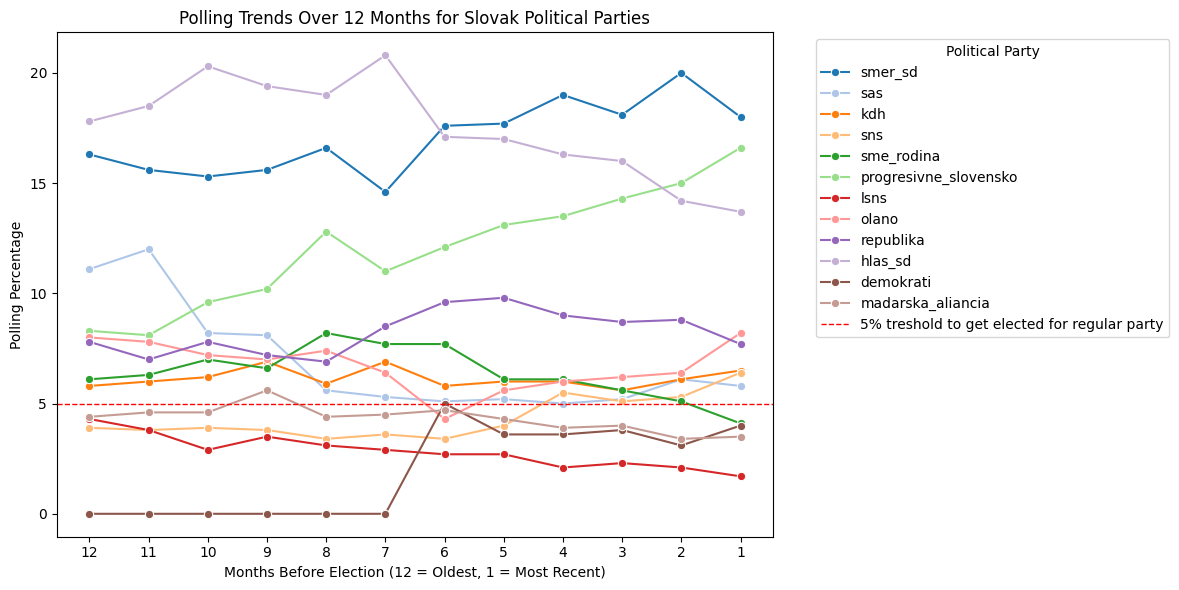
\includegraphics[width=\textwidth]{../images_exploratory/Polls_without_result_2023.png}
    \caption{}
    \label{fig:example}
\end{figure}

Už môžeme pozorovať ako sa vyvíjali názori voličov pred voľbami, napriklad zrod strany Demokrati alebo postupný prepad Hlasu či postupný nárast Progresivneho Slovenska.
Pridanie výsledku vo voľbách by malo ešte väčšiu výpovednú hodnotu, keďže budeme vedieť zhodnotiť aj to ako sa preferencie premietli už aj vo voľbách, a tak urobime presne to.
\begin{figure}[h]
    \centering
    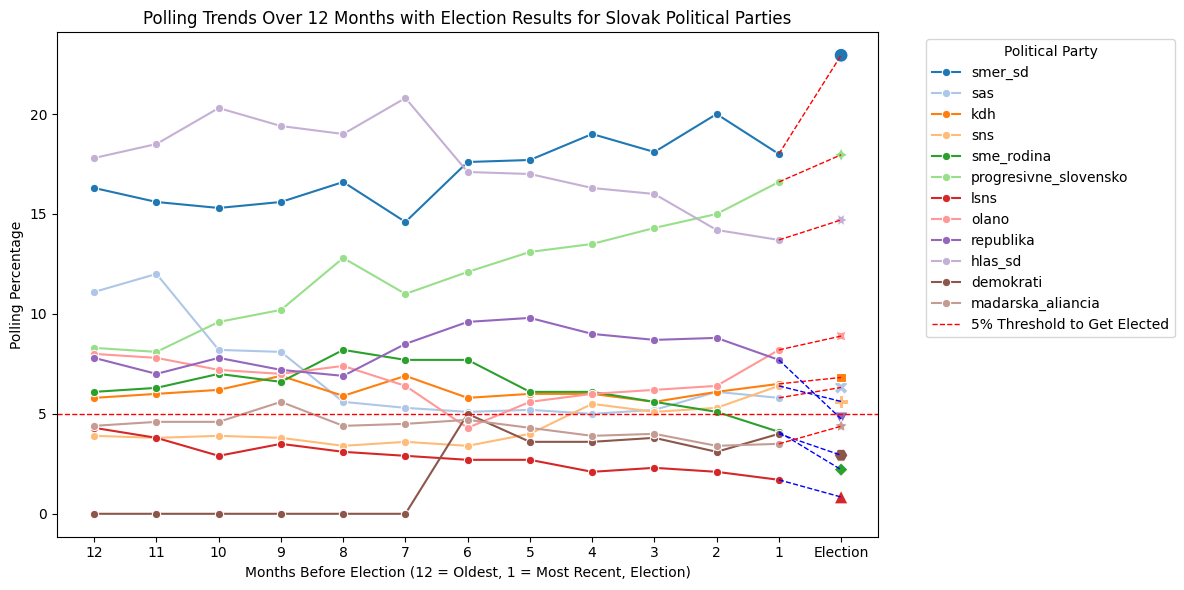
\includegraphics[width=\textwidth]{../images_exploratory/Polls_with_result_2023.png}
    \caption{}
    \label{fig:example}
\end{figure}

Teraz aj vidíme, že trendy v prieskumoch maju vplyv na to ako strana dopadne aj vo voľbách ale aj tu sa nájdu vynimky ako Hlas, ktorý padal ale nakoniec dopadol lepšie ako v posledných prieskumoch. Taktiež ak sa niektoré strany dostali až pod hranicu zvoliteľnosti v prieskumoch často ju už neprekonali. Voliči majú prirodzený strach, že im prepadne hlas, a tak práve takýto výsledok v prieskumoch môže veľmi ubližiť strane.

Toto bol pohľad len na predošle voľby ako vyzerali ale aj tie predtým?

\begin{figure}[h]
    \centering
    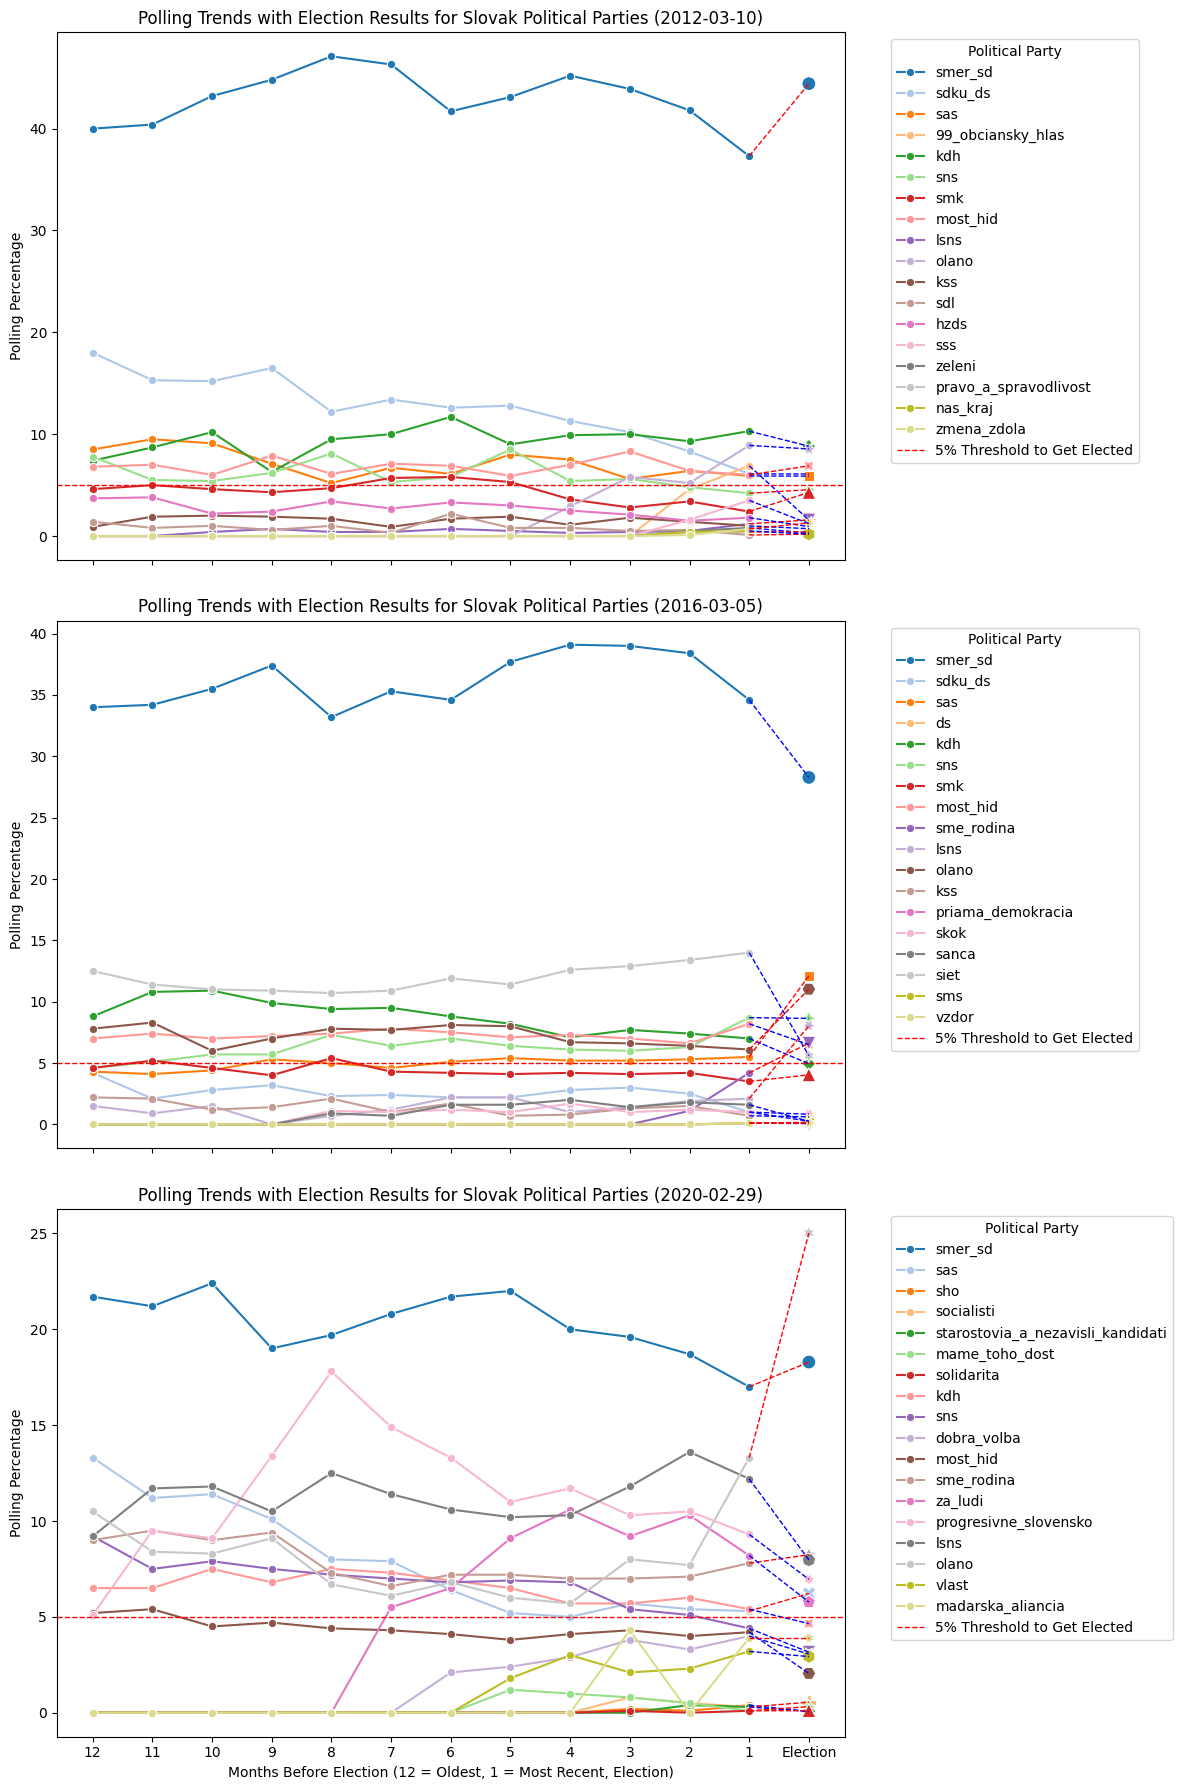
\includegraphics[width=\textwidth]{../images_exploratory/Polls_with_result_ALL.png}
    \caption{}
    \label{fig:example}
\end{figure}

OPIS GRAFU Nestiham haha

\subsection{Dopad predošleho vládnutia na voľby}

Rovnako v našich dátach je informacia o tom či v predošlom volebnom období bola daná strana súčasťou koalicie alebo bola v parlamente/opozicií. Bolo by teda vhodne sa pozrieť na to ako sa hýbali voličske zakladne od strán v koalicíi a strán ktoré v nej neboli. 
\begin{figure}[h]
    \centering
    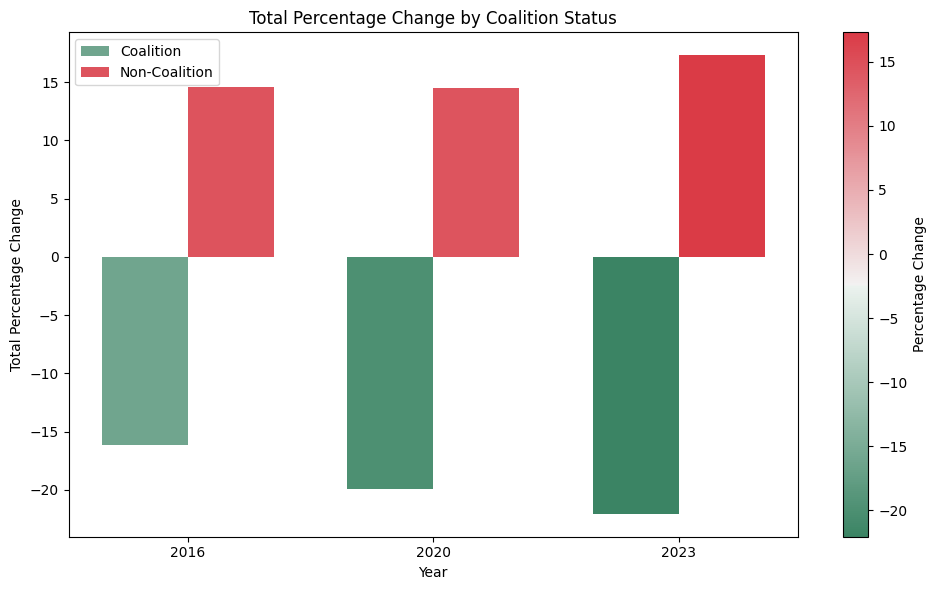
\includegraphics[width=\textwidth]{../images_exploratory/Coalition_vs_NoCoalition.png}
    \caption{}
    \label{fig:example}
\end{figure}
Strany, ktoré boli vo vláde, stratili často časť svojej voličskej základne, zatiaľ čo strany v opozícii mali tendenciu rásť. Tento jav naznačuje, že postavenie strany pred voľbami je relevantný faktor.



\end{document}
